\documentclass[runningheads]{llncs}

\usepackage[T1]{fontenc}
\usepackage{lmodern}
\usepackage{amsmath,amssymb}
\usepackage{booktabs}
\usepackage{array}
\usepackage{graphicx}
\usepackage{xcolor}
\usepackage{tikz}
\usetikzlibrary{arrows.meta,positioning,shapes.geometric,fit,backgrounds}
\usepackage{hyperref}
\hypersetup{hidelinks,colorlinks=true,allcolors=blue!60!black}


\newcommand{\method}{ESV-Gap}
\newcommand{\runid}{\texttt{deep\_learning\_\allowbreak iot\_intrusion\_\allowbreak de\_20260831\_\allowbreak 114802}}
\newcolumntype{L}[1]{>{\raggedright\arraybackslash}p{#1}}
\providecommand{\doi}[1]{}
\renewcommand{\doi}[1]{\href{https://doi.org/#1}{\texttt{\scriptsize doi:#1}}}

\begin{document}

\title{ESV-Gap: An Auditable Autonomous Reasoning Architecture for Evidence-Grounded Scientific Hypothesis Triage}
\titlerunning{Auditable Hypothesis Triage with ESV-Gap}

\author{Anh Hoa Le\thanks{Corresponding author.} \and Ly Van Khoa Phan \and Dinh Thanh Nguyen \and\\ Duc Hoang Nguyen \and Dinh Anh Ho \and Long Truong}
\authorrunning{A. H. Le et al.}
\institute{FPT University, Vietnam\\
\email{leanhhoa30012004@gmail.com, khoaplvse181656@fpt.edu.vn, thanhndse182854@fpt.edu.vn, hoangndse181655@fpt.edu.vn, anhhdse180670@fpt.edu.vn, longt5@fpt.edu.vn}}

\maketitle

\begin{abstract}
Autonomous machine intelligence (AMI) agents increasingly formulate scientific hypotheses by detecting associative patterns in literature, but can conflate representation sparsity with scientific novelty. We present \method{}, an auditable autonomous reasoning architecture executing a fail-closed epistemic control loop: \textbf{Observe} $\rightarrow$ \textbf{Hypothesize} $\rightarrow$ \textbf{Verify} $\rightarrow$ \textbf{Reason} $\rightarrow$ \textbf{Decide} $\rightarrow$ \textbf{Act/Abstain}. \method{} replaces naive graph sparsity heuristics with a Four-Pillar Evidence Verification engine: (A) two-stage external counterevidence verification decoupling lexical retrieval from semantic relation extraction; (B) source-disjoint author corroboration; (C) empirical extractor diagnostics reporting precision, recall, and miss rate with Wilson 95\% confidence intervals; and (D) corpus coverage diagnostics via Heaps' law and marginal discovery decay. In an empirical case study on deep-learning IoT intrusion detection (150 retained publications, 1,404 relation events, 1,185 canonical entities), \method{} triaged five post-gate candidate hypotheses. Stage A2 semantic verification, run with three open LLMs and resolved by majority vote, found verified counterevidence for three candidates ($60\%$); the other two were escalated to human review because their local corroboration was circular or absent, so no candidate was promoted to a research gap. The three models agreed on the counterevidence decision for 22 of 23 inspected records (Fleiss' $\kappa = 0.63$ over all four labels). On a small hand-built benchmark the extractor missed $38.9\%$ of gold relations ($95\%$ Wilson CI: $[24.8\%, 55.1\%]$), while canonical vocabulary growth ($\beta = 0.995$, discovery decay $-10.3\%$) established an unsaturated corpus. Across six deterministic fault-injection scenarios, \method{} enforced $100\%$ fail-closed abstention.

\keywords{Autonomous Machine Intelligence \and Evidence-Grounded Reasoning \and Scientific Discovery Agents \and Knowledge Graphs \and Hypothesis Triage \and Fail-Closed Systems.}
\end{abstract}

\section{Introduction}
\label{sec:intro}

Autonomous Machine Intelligence (AMI) aims to realize artificial agents capable of acquiring knowledge, reasoning over open-world dynamics, formulating hypotheses, and executing goal-directed plans with bounded human intervention~\cite{langley1987,king2009automation,lecun2022path}. While foundation models and agentic workflows enable automated discovery systems to scan literature and propose hypotheses at scale~\cite{aiscientist2024}, generative capacity has outpaced epistemic self-verification. Generating plausible conjectures is computationally cheap; determining whether a proposition represents a genuine open question, an already solved problem, an artifact of incomplete retrieval, or an extractor error is the central epistemic bottleneck~\cite{wadden2020scifact,schneider2022decade}.

When an autonomous agent constructs a scientific knowledge graph (KG), an absent edge between a method and an application can trigger a candidate research-gap hypothesis. Yet edge absence stems from multiple failure modes: unindexed external literature, relation extraction errors, terminology fragmentation, or abstract-level truncation. As Altman and Bland formulated, \emph{``Absence of evidence is not evidence of absence''}~\cite{altman1995absence}. Equating representation sparsity with scientific novelty can yield false-positive gap claims, duplicate research, and misallocated experimental effort.

We ask: \textbf{how can an autonomous agent determine whether an internally generated hypothesis is sufficiently supported by external evidence to act on, or whether it must abstain?}

We present \textbf{\method{}}, an auditable autonomous reasoning architecture for evidence-grounded hypothesis triage. Rather than treating hypothesis generation as an unconstrained generative task or defaulting to link prediction on a static graph, \method{} frames hypothesis triage as an active epistemic control loop:
\begin{equation}
\label{eq:loop}
\text{Observe} \longrightarrow \text{Hypothesize} \longrightarrow \text{Verify} \longrightarrow \text{Reason} \longrightarrow \text{Decide} \longrightarrow \text{Act/Abstain}
\end{equation}

\noindent\textbf{Key Contributions.} This work makes five primary contributions:
\begin{enumerate}\setlength{\itemsep}{0pt}\setlength{\topsep}{2pt}\setlength{\parsep}{0pt}\setlength{\partopsep}{0pt}
  \item \textbf{Two-Stage External Verification (Pillar A):} We decompose Pillar A into lexical candidate retrieval (Stage A1) and semantic relation extraction (Stage A2), preventing mere co-mentions of limitations from falsely refuting candidate gaps.
  \item \textbf{Strict Source-Disjoint Corroboration (Pillar B):} We require author-disjoint corroborating literature ($\mathcal{P}_{\text{cand}} \cap \mathcal{P}_{\text{corrob}} = \emptyset$), so circular citations cannot corroborate a candidate.
  \item \textbf{Diagnostic Reliability Characterization (Pillars C \& D):} We measure the extractor's miss rate on a gold benchmark ($n=36$, Wilson 95\% CIs) instead of assuming a global bound, and track canonical vocabulary growth via Heaps' law and marginal discovery decay.
  \item \textbf{Decoupled Epistemic Control Policy:} We separate disposition space $\mathcal{D}$ from action space $\mathcal{A}$ via a deterministic policy $\pi: \mathcal{D} \rightarrow \mathcal{A}$, providing an auditable, fail-closed abstention mechanism.
  \item \textbf{Empirical Auditability and Fault-Injection Validation:} We evaluate \method{} on 150 IoT cybersecurity publications with Stage A2 repeated across three LLMs, release record-level labels and evidence spans for every inspected document, and demonstrate 100\% fail-closed abstention across six predefined failure modes.
\end{enumerate}

\section{Related Work}
\label{sec:related}

\noindent\textbf{Autonomous Scientific Discovery and AMI.} Early symbolic systems such as BACON~\cite{langley1987} and the Robot Scientist Adam~\cite{king2009automation} executed closed-loop hypothesis generation and physical experimentation. In modern AMI, LeCun~\cite{lecun2022path} formalizes autonomous agents around perception, world modeling, reasoning, and objective-driven control. Recently, LLM-based systems such as The AI Scientist~\cite{aiscientist2024} demonstrated automated literature review and ideation, ResearchAgent~\cite{baek2025researchagent} and SciMON~\cite{wang2024scimon} generate ideas against retrieved prior work, and a human study judged LLM ideas more novel than expert ones~\cite{si2025ideas}; novelty is judged only against the papers that happen to be retrieved. Existing generative agents lack verifiable epistemic self-assessment and can accept unsupported or previously resolved gaps when external verification is absent.

\noindent\textbf{Graph-Theoretic Gap Discovery.} Knowledge graphs provide structured representations for literature synthesis and hypothesis discovery~\cite{swanson1986fish,schneider2022decade,chen2019ukge}. Most closely related to our work, Dachepally and Kandasamy~\cite{rahul2026dynamic} generated gap candidates using TransE link prediction, Louvain community detection~\cite{blondel2008fast}, and temporal activity decay. While their work offers valuable techniques for initial graph candidate generation, \method{} addresses the downstream verification problem: determining whether a structurally plausible candidate remains defensible after external retrieval, semantic counterevidence analysis, provenance checks, and corpus-coverage diagnostics.

\noindent\textbf{Scientific Claim Verification.} Claim verification frameworks, such as SciFact~\cite{wadden2020scifact} and SciFact-Open~\cite{wadden2022scifactopen}, evaluate natural-language assertions against corpora. However, these systems verify factual assertions (e.g., entity properties) rather than epistemic research gaps asserting that a capability has not been achieved. Verifying negative gap claims requires open-world external retrieval and semantic verification of whether retrieved papers resolve or merely discuss the challenge.

\noindent\textbf{Selective Classification and Fail-Closed Systems.} Fail-safe design~\cite{saltzer1975protection,shneiderman2020hcai} and selective classification with rejection~\cite{cortes2016learning,geifman2017selective} make abstention an explicit action under insufficient evidence. \method{} applies this principle: when probes fail, data is malformed, or corroboration is circular, the agent abstains and escalates to human review.

\section{Problem Formulation and Control Loop}
\label{sec:problem}

\subsection{Knowledge Graph and Attributed Relation Events}
Let $\mathcal{P} = \{p_1, \dots, p_N\}$ be a bounded corpus of ingested publications. We construct a multigraph $\mathcal{G} = (\mathcal{E}, \mathcal{R}, \mathcal{E}_{\text{events}})$ where $\mathcal{E}$ denotes canonical entities and $\mathcal{R}$ denotes directed relations (\texttt{ADDRESSES}, \texttt{USES}, \texttt{EVALUATES\_ON}, \texttt{IMPROVES}, \texttt{LACKS}, \texttt{APPLIED\_\allowbreak TO}). Each extracted instance is a \textbf{directed attributed relation event} $e = \langle u, r, v, p, y, c, q \rangle$, where $u, v \in \mathcal{E}$, $r \in \mathcal{R}$, $p \in \mathcal{P}$ is the source paper, $y \in \mathbb{N}$ is publication year, $c \in [0, 1]$ is confidence, and $q$ is the verbatim evidence span.

\subsection{Operational Hypothesis vs. Global Scientific Absence}
In naive graph discovery, an unobserved link between method $u$ and capability $v$ is asserted as an absolute gap: $\Phi_{\text{absent}}(u, v) \equiv \neg \exists e \in \mathcal{E}_{\text{events}} : \text{subj}(e) = u \wedge \text{rel}(e) = \texttt{ADDRESSES} \wedge \text{obj}(e) = v$. Such global absence claims cannot be established from a bounded corpus alone. We reformulate gap triage as an \textbf{operational verification claim}:
\begin{definition}[Operational Hypothesis Claim]
Given candidate gap $h = \langle u, \texttt{LACKS}, v \rangle$, external index family $\mathcal{S}$, query family $\mathcal{Q}(h)$, semantic verifier $\mathcal{V}$, and timestamp $t$, the machine-testable proposition is:
\begin{equation}
\label{eq:operational_claim}
\Phi_{\text{op}}(h) \equiv \text{Complete}(h) \wedge \left( \mathcal{C}_{\text{verified}}(h) = \emptyset \right) \wedge \left( |\mathcal{P}_{\text{disjoint}}(h)| \ge 1 \right)
\end{equation}
where $\mathcal{C}_{\text{verified}}$ is verified external counterevidence, $\mathcal{P}_{\text{disjoint}}$ is source-disjoint corroboration, and $\text{Complete}(h) \in \{0, 1\}$ indicates verification completion. Here, $\text{Complete}(h) = 1$ iff all configured index queries $\mathcal{S}$ and semantic checks $\mathcal{V}$ execute successfully without timeouts, HTTP 429 throttling, malformed JSON, or missing evidence spans. If any mandatory verification step fails, $\text{Complete}(h) = 0$, ensuring external failure cannot be conflated with evidence of absence.
\end{definition}

\subsection{Evidence, Dispositions, and Control Action Space}
Let $\mathbf{e}(h) = \langle \text{Complete}(h), |\mathcal{C}_{\text{verified}}(h)|, |\mathcal{P}_{\text{disjoint}}(h)|, \text{CorpusVerdict}(\mathcal{P}), R_{\text{ext}} \rangle$ denote the Four-Pillar evidence vector. Hypothesis triage is formalized via decision rule $\delta: \mathbf{e}(h) \rightarrow \mathcal{D}$ and action policy $a(h) = \pi(\delta(h))$ under fail-closed precedence:
\begin{equation}
\label{eq:disposition}
\delta(h) = \begin{cases}
\text{\scriptsize REFUTED}, & \text{if } |\mathcal{C}_{\text{verified}}(h)| \ge 1 \\
\text{\scriptsize REVIEW\_REQUIRED}, & \text{if } \text{Complete}(h) = 0 \;\vee\; |\mathcal{P}_{\text{disjoint}}(h)| < 1 \\
\text{\scriptsize EVIDENCE\_SUPPORTED}, & \text{if } \Phi_{\text{op}}(h) \wedge \text{CorpusVerdict}(\mathcal{P}) = \text{\scriptsize SATURATED} \\
\text{\scriptsize SUPPORTED\_OPEN}, & \text{if } \Phi_{\text{op}}(h) \wedge \text{CorpusVerdict}(\mathcal{P}) \ne \text{\scriptsize SATURATED}
\end{cases}
\end{equation}
The policy $\pi: \mathcal{D} \rightarrow \mathcal{A}$ executes: $\text{\scriptsize REFUTED} \mapsto \text{\scriptsize REJECT}$, $\text{\scriptsize REVIEW\_REQUIRED} \mapsto \text{\scriptsize ABSTAIN\_AND\_ESCALATE}$, $\text{\scriptsize EVIDENCE\_SUPPORTED} \mapsto \text{\scriptsize RETAIN\_AND\_FORMULATE}$, and $\text{\scriptsize SUPPORTED\_OPEN} \mapsto \text{\scriptsize RETAIN\_WITH\_WARNING}$. This establishes the closed loop $\mathbf{e}(h) \mapsto \delta(h) \mapsto a(h) = \pi(\delta(h))$. Because \texttt{REFUTED} has highest precedence, a single verified counterevidence record suffices for rejection regardless of completion status. If mandatory external verification remains incomplete and no verified counterevidence has already refuted the hypothesis, the decision rule returns \texttt{REVIEW\_REQUIRED} and triggers fail-closed abstention.

\section{\method{} Architecture}
\label{sec:arch}

The \method{} architecture operationalizes the epistemic loop of Eq.~(\ref{eq:loop}). As illustrated in Fig.~\ref{fig:arch}, the pipeline processes raw literature through structured observation, candidate generation, multi-stage verification, and policy execution.

\begin{figure}[t]
\centering
\resizebox{\columnwidth}{!}{%
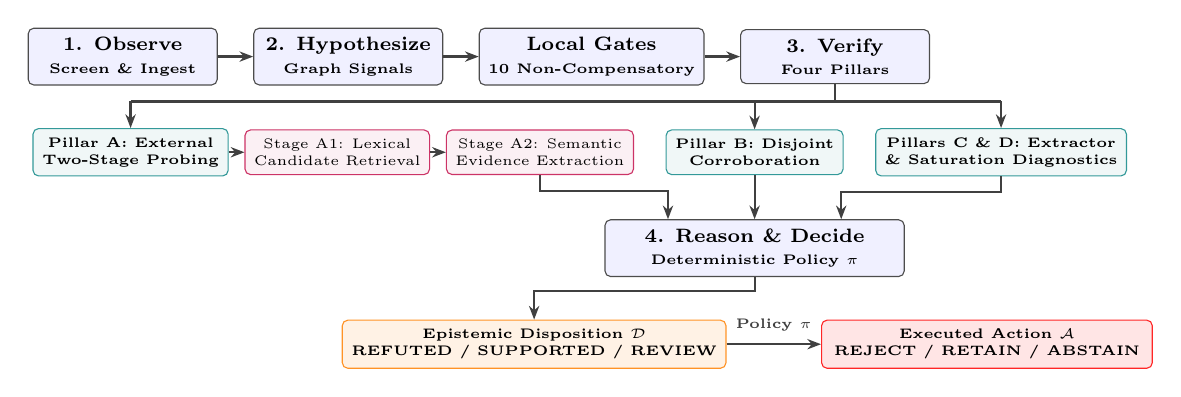
\begin{tikzpicture}[
  box/.style={rectangle, draw=black!70, fill=blue!6, rounded corners=2pt, minimum width=2.4cm, minimum height=0.54cm, font=\scriptsize\bfseries, align=center},
  stagebox/.style={rectangle, draw=purple!80, fill=purple!6, rounded corners=2pt, minimum width=1.95cm, minimum height=0.50cm, font=\tiny, align=center},
  pillar/.style={rectangle, draw=teal!80, fill=teal!6, rounded corners=2pt, minimum width=2.1cm, minimum height=0.52cm, font=\tiny\bfseries, align=center},
  disp/.style={rectangle, draw=orange!85, fill=orange!10, rounded corners=2pt, minimum width=4.2cm, minimum height=0.58cm, font=\tiny\bfseries, align=center},
  act/.style={rectangle, draw=red!85, fill=red!10, rounded corners=2pt, minimum width=4.2cm, minimum height=0.58cm, font=\tiny\bfseries, align=center},
  arrow/.style={-{Stealth[scale=0.75]}, thick, color=black!75},
  bus/.style={thick, color=black!75}
]

% Tier 1: Operational Loop
\node[box] (obs) {1. Observe\\ \tiny Screen \& Ingest};
\node[box, right=0.45cm of obs] (hyp) {2. Hypothesize\\ \tiny Graph Signals};
\node[box, right=0.45cm of hyp] (gates) {Local Gates\\ \tiny 10 Non-Compensatory};
\node[box, right=0.45cm of gates] (ver) {3. Verify\\ \tiny Four Pillars};

\draw[arrow] (obs) -- (hyp);
\draw[arrow] (hyp) -- (gates);
\draw[arrow] (gates) -- (ver);

% Tier 2: Verification Pillars
\node[pillar, below=0.54cm of obs, xshift=0.1cm] (pila) {Pillar A: External\\ Two-Stage Probing};
\node[stagebox, right=0.2cm of pila] (stg1) {Stage A1: Lexical\\ Candidate Retrieval};
\node[stagebox, right=0.2cm of stg1] (stg2) {Stage A2: Semantic\\ Evidence Extraction};
\draw[arrow] (pila) -- (stg1);
\draw[arrow] (stg1) -- (stg2);

\node[pillar, right=0.4cm of stg2] (pilb) {Pillar B: Disjoint\\ Corroboration};
\node[pillar, right=0.4cm of pilb] (pilcd) {Pillars C \& D: Extractor\\ \& Saturation Diagnostics};

% Clean Distribution Bus from 3. Verify to Pillars
\coordinate (splitY) at ([yshift=-0.22cm]ver.south);
\draw[bus] (ver.south) -- (splitY);
\draw[bus] (pila.north |- splitY) -- (pilcd.north |- splitY);
\draw[arrow] (pila.north |- splitY) -- (pila.north);
\draw[arrow] (pilb.north |- splitY) -- (pilb.north);
\draw[arrow] (pilcd.north |- splitY) -- (pilcd.north);

% Tier 3: Reasoning Box (centered under Pillar B)
\node[box, below=0.56cm of pilb, minimum width=3.8cm] (rsn) {4. Reason \& Decide\\ \tiny Deterministic Policy $\pi$};

% Clean Inputs into 4. Reason & Decide without line intersections
\draw[arrow] (stg2.south) -- ++(0,-0.20) -| ([xshift=-1.1cm]rsn.north);
\draw[arrow] (pilb.south) -- (rsn.north);
\draw[arrow] (pilcd.south) -- ++(0,-0.20) -| ([xshift=1.1cm]rsn.north);

% Tier 4: Disposition and Action (centered under rsn)
\node[disp, below=0.54cm of rsn, xshift=-2.8cm] (dspace) {Epistemic Disposition $\mathcal{D}$\\ \tiny REFUTED / SUPPORTED / REVIEW};
\node[act, right=1.2cm of dspace] (aspace) {Executed Action $\mathcal{A}$\\ \tiny REJECT / RETAIN / ABSTAIN};

\draw[arrow] (rsn.south) -- ++(0,-0.18) -| (dspace.north);
\draw[arrow] (dspace.east) -- node[above=1pt, font=\tiny\bfseries] {Policy $\pi$} (aspace.west);

\end{tikzpicture}%
}
\caption{\method{} Epistemic Control Loop, detailing the Two-Stage Pillar A verification engine and decoupling Epistemic Dispositions $\mathcal{D}$ from Executed Control Actions $\mathcal{A}$.}
\label{fig:arch}
\end{figure}

\subsection{Local Pre-Screening: Ten Non-Compensatory Validation Gates}
Candidate gap signals generated from the multigraph (via link-absence heuristics and community boundaries) must pass ten non-compensatory local gates: (1)~provenance, at least one anchor span; (2)~specificity, no generic or stop-word entities; (3)~no direct edge between $u$ and $v$; (4)~no subsumed link through taxonomy aliases; (5)~local semantic closure; (6)~at least two disjoint multigraph paths; survival of (7)~edge dropout ($\ge 0.70$), (8)~paper bootstrap ($\ge 0.65$) and (9)~plausible-edge additions ($\ge 0.60$); and (10)~domain alignment (similarity $\ge 0.75$). Failing gates reject the candidate, except Gate~5, which inspects sentence windows for action verbs (e.g., \emph{address}, \emph{mitigate}) not negated by cues such as \emph{struggle to address}, and escalates matches to \texttt{REVIEW\_\allowbreak REQUIRED} rather than pruning them. Surviving candidates are ranked by normalized publication recency.

\subsection{Pillar A: Two-Stage External Counterevidence Verification}
\label{sec:pillar_a}

A key failure mode in automated gap discovery is the false assumption that \textbf{lexical co-mention implies counterevidence}. For example, an abstract stating that zero-day attacks remain unresolved for deep-learning IDS co-mentions both terms but supports the limitation rather than refuting it.

To resolve this, we decompose Pillar A into two distinct stages:

\noindent\textbf{Stage A1: Lexical Candidate Retrieval.} The agent constructs boolean probe queries $Q_{\text{probe}}(u, v) = \texttt{"}u\texttt{" AND "}v\texttt{"}$ targeting external indexing services $\mathcal{S}$ (Semantic Scholar~\cite{semanticscholar2023} and OpenAlex~\cite{openalex2022}). The provider returns raw hit totals ($N_{\text{raw}}$). The agent paginates and fetches up to $K_{\text{fetch}} = 5$ recent records, extracting the title, abstract, authors, year, and persistent identifier (DOI, OpenAlex ID, Semantic Scholar ID). These records constitute the \textbf{Potential Counterevidence Pool}. Co-mention filtering at Stage A1 \emph{never} directly assigns a \texttt{REFUTED} disposition.

\noindent\textbf{Stage A2: Semantic Counterevidence Verification.} For each record in the Potential Counterevidence Pool, the agent extracts candidate evidence spans and assesses the semantic relation between method $u$ and capability $v$ with an instruction-tuned LLM using deterministic decoding ($\text{temperature} = 0.0$, seed 42; models in Sec.~\ref{sec:setup}). The model outputs a structured JSON schema: \texttt{classification}, \texttt{evidence\_}\allowbreak\texttt{span}, \texttt{confidence} $\in [0, 1]$, and \texttt{relation\_}\allowbreak\texttt{rationale}. Model-reported confidence is retained as audit metadata and does not directly enter the disposition policy; Stage A2 decisions are based on the categorical relation label together with verbatim evidence-span validation. We classify records into four mutually exclusive labels: (1)~\texttt{VERIFIED\_}\allowbreak\texttt{COUNTEREVIDENCE}, where the paper demonstrates, implements, or evaluates capability $v$ for method $u$ (relations \texttt{ADDRESSES}, \texttt{IMPROVES}, \texttt{EVALUATES\_}\allowbreak\texttt{ON}); (2)~\texttt{SUPPORTING\_}\allowbreak\texttt{LIMITATION}, where the paper identifies $v$ as an unresolved limitation (relation \texttt{LACKS}); (3)~\texttt{AMBIGUOUS}, discussing $u$ and $v$ without definitive resolution; or (4)~\texttt{IRRELEVANT}, reflecting superficial lexical co-occurrence. To prevent generative hallucinations, an automated verbatim substring check is enforced: an evidence span is mandatory for the two positive labels and must be an exact substring of the title or abstract; otherwise, the span is discarded as ungrounded. Persistent schema or network failure after 3 retries sets $\text{Complete}(h) = 0$, routing the candidate to \texttt{REVIEW\_REQUIRED} unless it is already \texttt{REFUTED}. Only records confirmed as \texttt{VERIFIED\_}\allowbreak\texttt{COUNTEREVIDENCE} with verified verbatim spans can contribute to a \texttt{REFUTED} disposition. For auditability, every verification record persists the exact quoted span, relation label, model confidence, DOI, and retrieval timestamp. When several verifier models are run, each record keeps one label per model and the candidate disposition is the majority over models.

\subsection{Pillar B: Source-Disjoint Author Corroboration}
To ensure that a surviving candidate is not an idiosyncratic claim from a single research group or an artifact of self-citation, Pillar B searches the retained local corpus ($\mathcal{P}$) for independent supporting publications asserting explicit research gaps (via extracted \texttt{LACKS} relation triples or curated gap phrase patterns). Let $\mathcal{P}_{\text{cand}}$ be the set of papers that originated the candidate gap. The candidate must be corroborated by a disjoint publication set: $\mathcal{P}_{\text{corrob}} \subseteq \mathcal{P}$ with $\mathcal{P}_{\text{corrob}} \cap \mathcal{P}_{\text{cand}} = \emptyset$ and $\text{Authors}(\mathcal{P}_{\text{corrob}}) \cap \text{Authors}(\mathcal{P}_{\text{cand}}) = \emptyset$. If all local supporting citations trace back to the candidate's origin publication, the corroboration is flagged as circular, failing the independence gate and forcing an immediate \texttt{REVIEW\_REQUIRED} disposition. External Stage A2 records are tracked independently and do not increment local corpus $N_{\text{corrob}}$.

\subsection{Pillar C: Extractor Diagnostic Reliability Characterization}
\label{sec:pillar_c}

An absent graph edge may simply reflect an extraction failure by the NLP pipeline. To quantify this risk, Pillar C runs the extractor on a small hand-annotated benchmark $\mathcal{D}_{\text{gold}}$ of 10 short abstract-style passages on explainable and secure machine learning, containing 36 gold relation events.

Let $TP$, $FP$, and $FN$ denote true positive, false positive, and false negative counts on the diagnostic benchmark. The empirical metrics are $\text{Precision} = \frac{TP}{TP + FP}$, $\text{Recall} = \frac{TP}{TP + FN}$, and $F_1 = \frac{2 \cdot \text{Precision} \cdot \text{Recall}}{\text{Precision} + \text{Recall}}$. The empirical extractor miss rate is $\text{MissRate} = 1 - \text{Recall} = \frac{FN}{TP + FN}$. For each binomial proportion we report a two-sided 95\% Wilson score interval~\cite{wilson1927}, with denominators $TP + FN$ for recall and miss rate and $TP + FP$ for precision.

\noindent\textbf{Empirical Interpretation.} Rather than asserting unverified Bayesian inequalities across unobserved document distributions, the benchmark provides an empirical diagnostic estimate: for the pipeline's extraction model, $\hat{P}(\text{miss} \mid \text{present}) = 14/36 \approx 38.9\%$ ($95\%$ Wilson CI: $[24.8\%, 55.1\%]$). Pillar C does not enter $\delta(h)$ as a heuristic multiplier; it serves as a diagnostic epistemic qualifier: characterizing a known source of representational uncertainty and empirically motivating why external verification (Pillar A) and source-disjoint corroboration (Pillar B) are mandatory before accepting any gap.

\subsection{Pillar D: Corpus Vocabulary Saturation Diagnostics}
To evaluate whether the ingested corpus $\mathcal{P}$ adequately covers the domain's conceptual space, Pillar D tracks canonical vocabulary expansion using Heaps' law~\cite{heaps1978}: $\mathcal{V}(n) = K \cdot n^\beta$, where $n$ is cumulative ingested papers, $\mathcal{V}(n)$ is unique canonical entities, and $\beta$ is the growth exponent estimated via log-log ordinary least squares. We measure marginal discovery decay between the initial and final quintiles ($q = 30$ papers): $\Delta_{\text{decay}} = 1 - M_{\text{final}} / M_{\text{initial}} = (M_{\text{initial}} - M_{\text{final}}) / M_{\text{initial}}$, where $M$ denotes mean new canonical entities discovered per paper. Positive $\Delta_{\text{decay}}$ indicates decelerating discovery (decay), whereas negative values reflect expanding discovery. We categorize corpus coverage using predefined operational heuristic thresholds: (1)~\textbf{SATURATED:} $\beta < 0.65$ and $\Delta_{\text{decay}} \ge 0.60$ (sublinear flattening; local corpus absence is less likely to be attributable to ongoing vocabulary expansion); (2)~\textbf{MATURING:} $\beta < 0.80$ and $\Delta_{\text{decay}} \ge 0.30$ (moderate conceptual growth); and (3)~\textbf{UNSATURATED:} $\beta \ge 0.80$ or $\Delta_{\text{decay}} < 0.30$ (incoming literature actively introduces novel concepts; open-world corpus). When a corpus is diagnosed as \texttt{UNSATURATED}, the agent is prohibited from issuing an absolute gap claim, qualifying surviving candidates as \texttt{SUPPORTED\_OPEN}.

\section{Experimental Setup}
\label{sec:setup}

\noindent\textbf{Target Domain and Ingestion Corpus.} We evaluate \method{} on deep-learning Internet-of-Things (IoT) intrusion detection systems (IDS), spanning publications from 2019 to 2026. The initial ingestion harvested 600 candidate records from scholarly index APIs. Domain-specific automated screening (IoT edge architectures, machine learning classifiers, and threat detection) yielded 192 candidate papers. Following full-text accessibility verification and duplicate removal, $N = 150$ retained scholarly publications formed the primary study corpus.

\noindent\textbf{Model Implementations and Hyperparameters.} The pipeline is configured for relation extraction with gpt-oss-20b served by Groq (structured JSON output, exponential backoff, up to 3 retries); the frozen run did not record the model identifier, and the Pillar C evaluation runs this configured model and gpt-oss-120b at temperature 0. Domain relevance screening applied a confidence threshold $\tau_{\text{conf}} = 0.70$: papers whose LLM-assigned relevance score fell below this threshold were excluded from the retained corpus. Stage A2 was run with three open models served by Groq, gpt-oss-120b, gpt-oss-20b and Qwen3.8-27B (temperature 0, seed 42, JSON output), on the Stage A1 records of the frozen run; it applies no confidence cutoff, records model confidence as audit metadata, and enforces verbatim substring matching against retrieved titles and abstracts before admitting evidence spans. Llama-3.3-70B, used in earlier experiments with this pipeline, is no longer served and was not used for the reported results. Louvain community detection used resolution $\gamma = 1.0$ (seed 42). Entity canonicalization combined TF-IDF cosine similarity (threshold 0.75) with lexical normalizers. OpenAlex~\cite{openalex2022} and Semantic Scholar~\cite{semanticscholar2023} were probed for up to $K_{\text{fetch}} = 5$ records per candidate query; OpenAlex returned no records for these queries, so all inspected records come from Semantic Scholar (frozen experiment run identifier: \path{deep_learning_iot_intrusion_de_20260831_114802}).

\noindent\textbf{Research Questions.} \textbf{RQ1} extractor precision, recall and miss rate on $\mathcal{D}_{\text{gold}}$; \textbf{RQ2} corpus saturation; \textbf{RQ3} fail-closed abstention under faults; \textbf{RQ4} counterevidence versus limitation co-mentions; \textbf{RQ5} candidate filtering across pillars.

\section{Results}
\label{sec:results}

\subsection{Extractor Diagnostic Evaluation (RQ1)}
The relation extractor identified 1,404 directed attributed relation events across 1,185 canonical entities in the 150-paper corpus. Table~\ref{tab:gold} reports performance on the 36-triple expert gold benchmark $\mathcal{D}_{\text{gold}}$.

\begin{table}[htbp]
\centering
\caption{Extractor Diagnostic Evaluation on Gold Benchmark $\mathcal{D}_{\text{gold}}$ ($n = 36$) for the configured extraction model (gpt-oss-20b) and a larger model (gpt-oss-120b).}
\label{tab:gold}
\scriptsize
\setlength{\tabcolsep}{3pt}
\renewcommand{\arraystretch}{0.92}
\begin{tabular}{lccccc}
\toprule
 & & \multicolumn{2}{c}{\textbf{gpt-oss-20b}} & \multicolumn{2}{c}{\textbf{gpt-oss-120b}} \\
\cmidrule(lr){3-4}\cmidrule(lr){5-6}
\textbf{Relation Category} & \textbf{Gold} & \textbf{TP} & \textbf{Recall} & \textbf{TP} & \textbf{Recall} \\
\midrule
\texttt{ADDRESSES} & 8 & 5 & 62.5\% & 6 & 75.0\% \\
\texttt{USES} & 8 & 4 & 50.0\% & 5 & 62.5\% \\
\texttt{LACKS} (Limitations) & 6 & 4 & 66.7\% & 5 & 83.3\% \\
\texttt{EVALUATES\_ON} & 4 & 2 & 50.0\% & 3 & 75.0\% \\
\texttt{IMPROVES} & 4 & 4 & 100.0\% & 4 & 100.0\% \\
\texttt{APPLIED\_TO} & 3 & 2 & 66.7\% & 2 & 66.7\% \\
\texttt{COMPARES} & 2 & 0 & 0.0\% & 0 & 0.0\% \\
\texttt{CONTRADICTS} & 1 & 1 & 100.0\% & 0 & 0.0\% \\
\midrule
\textbf{Total} (TP / FN / FP) & \textbf{36} & \multicolumn{2}{c}{\textbf{22 / 14 / 8}} & \multicolumn{2}{c}{\textbf{25 / 11 / 14}} \\
Recall [95\% CI] & & \multicolumn{2}{c}{61.1\% [44.9, 75.2]} & \multicolumn{2}{c}{69.4\% [53.1, 82.0]} \\
Precision [95\% CI] & & \multicolumn{2}{c}{73.3\% [55.6, 85.8]} & \multicolumn{2}{c}{64.1\% [48.4, 77.3]} \\
Miss rate [95\% CI] & & \multicolumn{2}{c}{38.9\% [24.8, 55.1]} & \multicolumn{2}{c}{30.6\% [18.0, 46.9]} \\
\bottomrule
\end{tabular}
\end{table}

With the configured extraction model, recall on $\mathcal{D}_{\text{gold}}$ was $61.1\%$ (22/36), precision $73.3\%$ (22/30) and $F_1$ $66.7\%$; the miss rate was $38.9\%$ ($95\%$ Wilson CI: $[24.8\%, 55.1\%]$). The larger model missed $30.6\%$ ($[18.0\%, 46.9\%]$) at lower precision. Both models missed every \texttt{COMPARES} relation. Roughly one gold relation in three was missed, so missing graph edges cannot be read as scientific gaps without external verification. Because $\mathcal{D}_{\text{gold}}$ consists of short constructed passages outside the IoT domain, these rates characterize the extractor rather than bound its error on the study corpus.

\subsection{Corpus Coverage Diagnostics (RQ2)}
Figure~\ref{fig:saturation} depicts vocabulary accumulation and marginal discovery across the 150-paper corpus.

\begin{figure}[t]
\centering
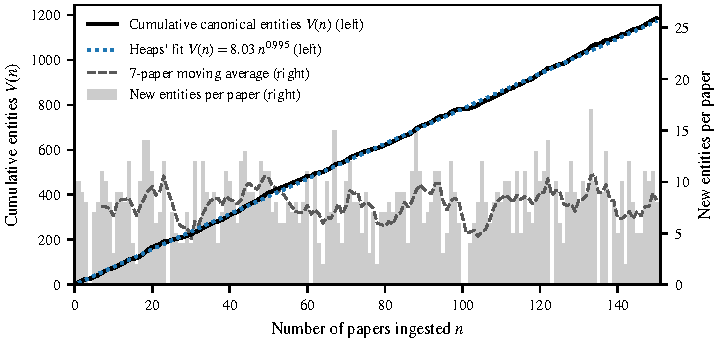
\includegraphics[width=\textwidth]{figures/corpus_saturation_curve.pdf}
\caption{Corpus vocabulary growth across 150 IoT cybersecurity publications: cumulative canonical entities (solid) with Heaps' fit (dotted, left axis), and new entities per paper (grey bars) with a 7-paper moving average (dashed, right axis); $V_{\text{observed}}(150) = 1{,}185$. Heaps' law fit yields $\beta = 0.995$ ($R^2 = 0.9983$) and discovery decay $\Delta_{\text{decay}} = -10.3\%$, diagnosing the literature as \texttt{UNSATURATED}.}
\label{fig:saturation}
\end{figure}

The initial quintile ($q = 30$ papers) introduced $M_{\text{initial}} = 7.43$ new canonical entities per paper and the final quintile $M_{\text{final}} = 8.20$, so $\Delta_{\text{decay}} = -10.3\%$: discovery accelerated rather than saturating. Log-log regression yielded a Heaps' law scaling parameter of $K = 8.0315$ and growth exponent $\beta = 0.9946 \approx 0.995$ ($R^2 = 0.9983$). (Evaluating pre-canonicalization raw mentions similarly demonstrated open growth: $V = 1,396, \beta = 1.037, \Delta_{\text{decay}} = -18.6\%$). Because $\beta \ge 0.80$ and $\Delta_{\text{decay}} < 0.30$, Pillar D assigned the operational verdict \texttt{UNSATURATED}. This diagnostic prohibits claiming global scientific absence, qualifying surviving hypotheses as open-world propositions.

\subsection{Two-Stage Semantic Verification and Candidate Triage (RQ4)}
The ten local validation gates filtered initial graph signals down to five post-gate candidate hypotheses (C1--C5). Table~\ref{tab:triage} tracks these candidates across the two-stage external verification pipeline. Stage A2 was applied to every inspected record, not only to lexical co-mentions, and repeated with three models. Table~\ref{tab:evidence} presents one auditable evidence span per candidate.

\begin{table}[htbp]
\centering
\caption{Two-Stage External Verification and Candidate Triage on Post-Gate Candidates.}
\label{tab:triage}
\scriptsize
\setlength{\tabcolsep}{2.0pt}
\begin{tabular}{p{0.4cm}p{2.5cm}cccccp{1.6cm}p{1.2cm}}
\toprule
\textbf{ID} & \textbf{Candidate Hypothesis} & \textbf{Raw} & \textbf{Insp} & \textbf{Co-M} & \textbf{Counter.} & \textbf{Corrob} & \textbf{Disposition $\mathcal{D}$} & \textbf{Action $\mathcal{A}$} \\
\midrule
C1 & Deep learning IoT IDS $\rightarrow$ Zero-day attacks & 864 & 5 & 5 & 5/5/5 & 0 & \texttt{REFUTED} & \texttt{REJECT} \\
C2 & Deep learning IoT IDS $\rightarrow$ Standardized protocols & 400 & 4$^\dagger$ & 4 & 0/0/0 & 0$^*$ & \texttt{REVIEW\_REQ} & \texttt{ABSTAIN} \\
C3 & Deep learning IoT IDS $\rightarrow$ Real-world industrial validation & 146 & 4$^\dagger$ & 4 & 0/1/0 & 0 & \texttt{REVIEW\_REQ} & \texttt{ABSTAIN} \\
C4 & ML IoT IDS $\rightarrow$ Edge computational overhead & 189 & 5 & 0 & 4/4/4 & 3 & \texttt{REFUTED} & \texttt{REJECT} \\
C5 & ML IoT IDS $\rightarrow$ Adversarial attack defenses & 1095 & 5 & 5 & 2/2/2 & 0 & \texttt{REFUTED} & \texttt{REJECT} \\
\bottomrule
\multicolumn{9}{p{11.5cm}}{\tiny Counter: records labeled \texttt{VERIFIED\_COUNTEREVIDENCE} with a verbatim span by gpt-oss-120b / gpt-oss-20b / Qwen3.8-27B. $^\dagger$Stage A1 inspected five records; the run stored identifiers for the four co-mentions only. $^*$C2 has one local corroborating citation, from the candidate's own source paper (circular provenance).}
\end{tabular}
\end{table}

\begin{table}[htbp]
\centering
\caption{Auditable Bibliographic Evidence Table for Central External and Corroborating Publications.}
\label{tab:evidence}
\tiny
\setlength{\tabcolsep}{2.5pt}
\renewcommand{\arraystretch}{0.82}
\begin{tabular}{L{0.4cm}L{1.4cm}L{2.4cm}L{2.1cm}L{4.9cm}}
\toprule
\textbf{ID} & \textbf{Citation} & \textbf{Publication Title} & \textbf{Identifier / Venue} & \textbf{Verbatim Evidence Span (Stage A2 label, votes)} \\
\midrule
C1 & Nitrat et al.~\cite{nitrat2025zeroday} & Zero-Day Attack Detection in IoT Networks\dots & DOI: 10.1109/\allowbreak OJCOMS.2025.\allowbreak 3604826 & \emph{``In zero-day scenarios, CZ-ResViT achieved 82\% accuracy on CIC IoT 2023 and 81\% on IoTID20, outperforming other DL models\dots''} (Counterevidence, 3/3) \\
\midrule
C2 & Shukla et al.~\cite{shukla2025effective} & An effective hybrid deep learning metaheuristic\dots & DOI: 10.1007/\allowbreak s10791-025-\allowbreak 09708-w & \emph{``The high diversity of IoT devices, their protocols and standards, and their limited computational resources have led to the appearance of novel security challenges.''} (Supporting limitation, 2/3) \\
\midrule
C3 & Tsallis et al.~\cite{tsallis2026industrial} & Industrial Wireless Networks in Industry 4.0\dots & DOI: 10.3390/\allowbreak jsan15010007 & \emph{``However, gaps remain in mobility support, interoperability across protocol layers, and field validation.''} (Supporting limitation, 3/3) \\
\midrule
C4 & Kamruzzaman et al.~\cite{kamruzzaman2025lightweight} & Lightweight AI-Driven Intrusion Detection for SMEs\dots & DOI: 10.1177/\allowbreak 18724981251398354 & \emph{``\dots tree-based ensemble models\dots achieved superior detection performance while maintaining minimal computational cost.''} (Counterevidence, 3/3) \\
\midrule
C5 & Nguyen et al.~\cite{nguyen2025adversarial} & Adversarial Attack and Defense in AI-Powered IDS & DOI: 10.15625/\allowbreak 1813-9663/\allowbreak 22884 & \emph{``\dots we propose APELID+, an enhanced IDS framework integrating adversarial training and feature squeezing techniques to effectively counter AML threats.''} (Counterevidence, 3/3) \\
\bottomrule
\end{tabular}
\end{table}

\noindent\textbf{Analysis of Candidate Triage Outcomes.} Multi-pillar verification resolved the five candidates into two outcomes (Tables~\ref{tab:triage} and~\ref{tab:evidence}).
(1)~\emph{Refutations (C1, C4, C5):} all three models labeled records as verified counterevidence: five for C1 (e.g., 82\% zero-day accuracy~\cite{nitrat2025zeroday}), two for C5 (adversarial training against AML threats~\cite{nguyen2025adversarial}) and four for C4, whose records evaluate lightweight intrusion detectors with low computational cost~\cite{kamruzzaman2025lightweight}. C4 had no lexical co-mention under its strict query phrases, and three independent 2026 papers in the corpus still describe computational cost as a limitation~\cite{jenish2026review,alam2026reservoir,mahdi2026scf}; because \texttt{REFUTED} has precedence, external counterevidence outweighs this local corroboration.
(2)~\emph{Escalations (C2, C3):} no record was counterevidence by majority. For C2, external records describe protocol diversity only as an obstacle~\cite{shukla2025effective}, and Pillar~B traced the single local corroboration back to the candidate's origin paper (\texttt{04b3ca64}). For C3, one model labeled one record as counterevidence and the other two did not; the records describe field validation as open~\cite{tsallis2026industrial}, but the corpus contains no independent corroboration. Both candidates were routed to \texttt{REVIEW\_REQUIRED} $\rightarrow$ \texttt{ABSTAIN\_AND\_ESCALATE}.

\noindent\textbf{Retrieval-Depth Robustness ($K_{\text{fetch}}$ Sensitivity).} Under a fixed ranking, a larger $K_{\text{fetch}}$ inspects a superset of records and can only add counterevidence, so the \texttt{REFUTED} dispositions of C1, C4 and C5 cannot be reversed by deeper retrieval. We re-ran Stage A2 (gpt-oss-120b and -20b) on the top 50 Semantic Scholar records of the same queries for C2 (retrieved October 2026) and C4 (cached a day after the run). C2 received no counterevidence from either model at $K = 5, 10, 20, 50$, so its escalation does not depend on retrieval depth. For C4, counterevidence grew with depth (4, 6, 12--13 and 24--25 records at $K = 5, 10, 20, 50$), confirming the refutation. C3 was not re-probed at depth.

\noindent\textbf{Execution Cost.} Stage~A2 issues one LLM call per inspected record, 23 calls per model for the cohort. Mean latency was 3.7--4.2\,s per call, and one model used 12.8k--14.3k prompt and 2.4k--4.3k completion tokens for all 23 records. Cost grows linearly with $K_{\text{fetch}}$ and the number of candidates.

\subsection{Pipeline Ablation Analysis (RQ5)}
Table~\ref{tab:ablation} traces the progressive filtering of candidate hypotheses across each stage of the \method{} pipeline.

\begin{table}[htbp]
\centering
\caption{Component-Level Pipeline Ablation across Post-Gate Candidates ($n = 5$).}
\label{tab:ablation}
\scriptsize
\setlength{\tabcolsep}{2pt}
\renewcommand{\arraystretch}{0.78}
\begin{tabular}{lccccL{4.3cm}}
\toprule
\textbf{Pipeline Stage} & \textbf{Eligible} & \textbf{Refuted} & \textbf{Review} & \textbf{Retained} & \textbf{Interpretation} \\
\midrule
Local gates only & 5 & 0 & 0 & 5 & Graph sparsity alone promotes all 5 candidates. \\
Co-mention baseline$^\dagger$ & 1 & 4 & 0 & 1 & Refutes C2 and C3 without counterevidence and promotes C4. \\
+ Pillar A (A1+A2) & 2 & 3 & 0 & 2 & Semantic verification refutes C1, C4, C5 and keeps C2, C3. \\
+ Pillar B & 0 & 3 & 2 & 0 & C2 circular, C3 uncorroborated: fail-closed abstention. \\
+ Pillars C \& D & 0 & 3 & 2 & 0 & No surviving candidate to qualify. \\
\bottomrule
\multicolumn{6}{p{\linewidth}}{\tiny $^\dagger$Counterfactual naive lexical matching rule (not \method{} policy).}
\end{tabular}
\end{table}

Without external verification, relying solely on graph sparsity promotes all five candidates. Stage~A2 refuted three ($60\%$) and Pillar~B escalated the remaining two, so none was promoted. The lexical co-mention baseline errs in both directions: it refutes C2 and C3 without any counterevidence, and it keeps C4, for which four of five inspected records report lightweight detectors with low computational cost.

\subsection{Fail-Closed Fault-Injection Validation (RQ3)}
We injected six deterministic failures into the decision engine: (1)~index timeout after retries, (2)~HTTP 429 throttling, (3)~incomplete pagination, (4)~malformed JSON, (5)~corroboration consisting only of self-citations, and (6)~a candidate without supporting paper identifiers. All six ($100\%$) produced \texttt{REVIEW\_REQUIRED} $\rightarrow$ \texttt{ABSTAIN\_AND\_ESCALATE}, so no failure led to an ungrounded claim. Scenario~6 initially failed, because the engine let independent corroboration stand in for local provenance; it passes after the fix in the released code.

\noindent\textbf{Heaps' Law Parameter Sensitivity.} Corpus coverage classification was evaluated across $\beta_{\text{thresh}} \in [0.65, 0.85]$ and $\Delta_{\text{decay, thresh}} \in [0.10, 0.40]$. Across all configurations, the empirical values ($\beta = 0.995$, $\Delta_{\text{decay}} = -10.3\%$) remained in the \texttt{UNSATURATED} region.

\section{Threats to Validity and Limitations}
\label{sec:threats}

\noindent\textbf{Diagnostics, Verification, and Canonicalization.} Gold benchmark $\mathcal{D}_{\text{gold}}$ (36 triples in 10 short constructed passages outside the IoT domain) demonstrates that extraction error is substantial, rather than providing a bound for the study corpus; its Wilson interval for the miss rate spans 30 percentage points, and a benchmark of at least 100 triples drawn from the study corpus is needed for a tighter estimate. Furthermore, Stage~A2 semantic verification has not yet been evaluated against an independent, human-annotated external-evidence benchmark; classification error could alter candidate labeling between \texttt{REFUTED} and supporting or ambiguous categories, and model-reported confidence values are not calibrated probabilities. Agreement among three LLMs ($\kappa = 0.63$; 22/23 identical counterevidence decisions) measures consistency, not accuracy, and each refutation rests on verbatim spans that readers can check (Table~\ref{tab:evidence}). Hosted models also change over time: Llama-3.3-70B, used in earlier experiments, is no longer served, so per-record labels are released to let dispositions be re-derived. The frozen run did not record its extraction model, and for C2 and C3 one inspected record per candidate has no stored identifier. In addition, boolean query generation and entity canonicalization rely on lexical normalization and TF-IDF similarity, which are vulnerable to synonym drift, abbreviations, and terminology fragmentation across subfields. This is likely harder outside cybersecurity, e.g.\ in biomedicine, where genes and diseases carry many aliases and query expansion would need controlled vocabularies such as MeSH.

\noindent\textbf{Retrieval Scope, Scale, and Temporal Bounds.} Scholarly APIs (Semantic Scholar, OpenAlex) and top-$K$ rankings are not exhaustive, though C2 remained without counterevidence up to $K=50$ under default ranking; Stage A2 was run in October 2026 on records retrieved in September 2026, and OpenAlex returned no records for our queries. Our empirical evaluation examined $n=5$ post-gate hypotheses across 150 IoT cybersecurity papers; reported triage proportions ($60\%$ refuted, none promoted) are descriptive case-study statistics rather than population estimates, and cross-domain generalization remains unevaluated. A larger candidate set and a second domain such as biomedicine are needed before these proportions can be generalized. External probes analyzed titles and abstracts, potentially omitting evidence reported solely in full text or appendices. Finally, gap triage reflects timestamped literature states that evolve as new publications appear.

\section{Conclusion}
\label{sec:conclusion}

We presented \textbf{\method{}}, an auditable autonomous reasoning architecture for evidence-grounded hypothesis triage. By executing an active epistemic control loop with Four-Pillar Evidence Verification, \method{} replaces graph sparsity heuristics with empirical verification. In an empirical case study on deep-learning IoT intrusion detection (150 publications, 1,404 relation events), \method{} refuted three of five candidate gaps with counterevidence verified by a majority of three LLMs, escalated the other two because their corroboration was circular or absent, and promoted none. Across six predefined fault-injection scenarios, the architecture enforced fail-closed abstention without ungrounded conjecture, demonstrating how explicit epistemic constraints prevent autonomous scientific reasoning pipelines from promoting unsupported hypotheses when evidence is incomplete, contradictory, or provenance-limited.

\begin{credits}
\subsubsection{\ackname} This study received no external funding.

\subsubsection{Use of Generative AI.} Besides the LLMs that are part of the method (Sec.~\ref{sec:setup}), the authors used Claude (Anthropic) to help write analysis code and edit the manuscript. The authors checked all code, numbers and text and take full responsibility for the content.

\subsubsection{\discintname}
The authors have no competing interests to declare that are relevant to the content of this article.
\end{credits}

\bibliographystyle{splncs04}
\bibliography{references}

\end{document}
